\documentclass[../main.tex]{subfiles}
\graphicspath{{\subfix{../images/}}} % Images path

\begin{document}

\section{Dataset Description}\label{sec:dataset-description}

The dataset used in this study is the \textit{15-Scenes} dataset from
\textit{Lazebnik et al.}~\cite{lazebnik}.
This dataset consists of a total of $4485$ grayscale images, each belonging to
one of $15$ different scene categories
(\itt{Office,
	Kitchen,
	LivingRoom,
	Bedroom,
	Store,
	Industrial,
	TallBuilding,
	InsideCity,
	Street,
	Highway,
	Coast,
	OpenCountry,
	Mountain,
	Forest,
	Suburb}). 
The images are divided into a training set of $1500$ images, with $100$ images
per category, and a test set of $2985$ images with a non-uniform distribution as
shown in Figure~\ref{fig:dataset-distribution}.\\
Moreover, it's worth mentioning that the images in the dataset have different sizes and aspect ratios, with the majority of them being $256 \times 256$ pixels. 

\begin{figure}[H]
  \centering
  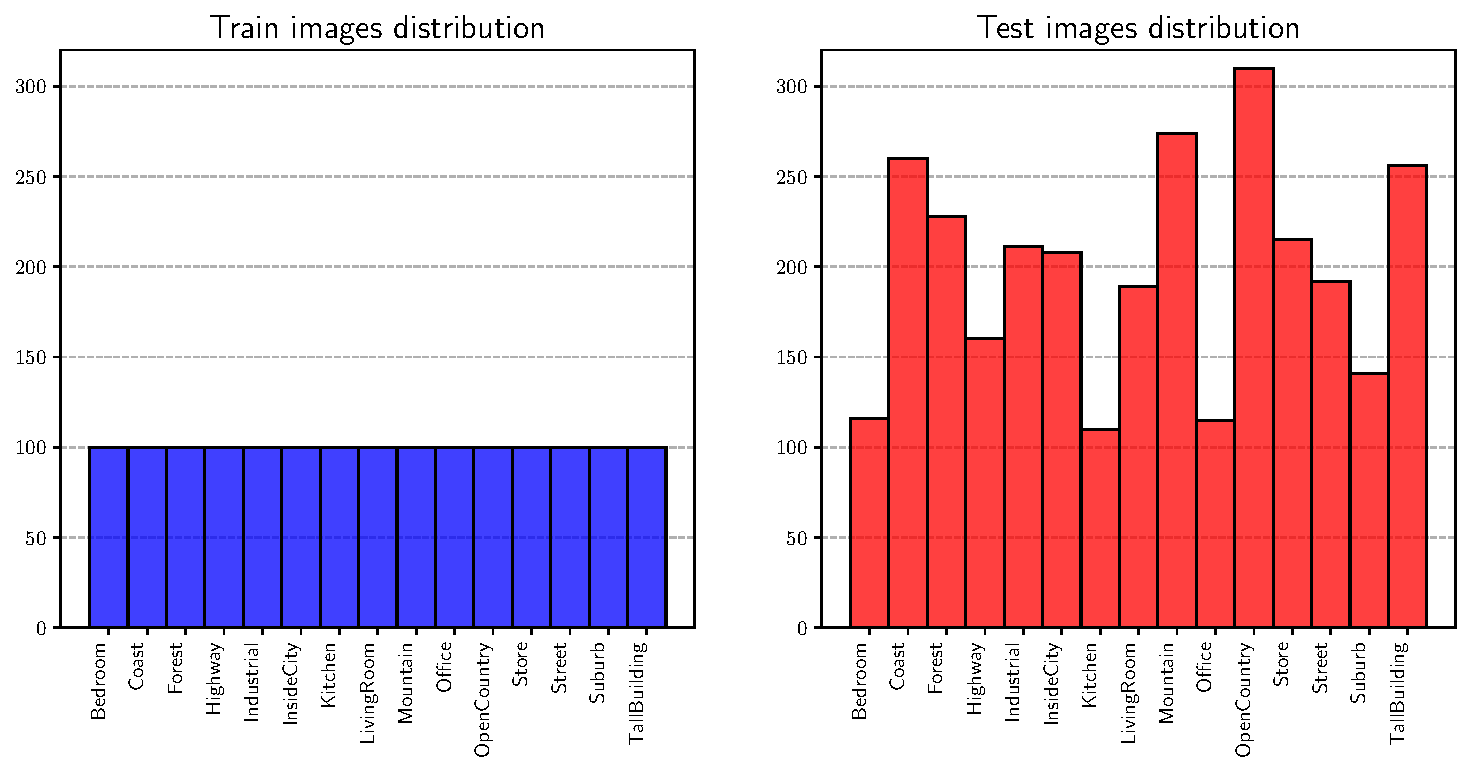
\includegraphics[width=\textwidth]{classes_distribution.pdf}
  \caption{Distribution of images in train (\itt{blue}) and test (\itt{red}) sets.}
  \label{fig:dataset-distribution}
\end{figure}

\end{document}
